\section[CLAIX-2023 GPU at RWTH Aachen University]{CLAIX-2023 GPU at RWTH Aachen University \hyperref[tab:examples-overview]{$\uparrow$}}
\label{sec:example-rwth-claix-2023-gpu}

The CLAIX-2023 cluster went into production at RWTH Aachen University in December 2023.
The GPU partition features 52 nodes each with two Intel Xeon 8468 Sapphire Rapids CPUs and four NVIDIA Tesla H100 Hopper GPUs.
While most on-node compute components are direct liquid cooled by two rack-external \acp{CDU}, seven side coolers are also placed inbetween racks.
These \acp{CDU} and side coolers are referred to as cooling components in the following.
Computes nodes of CLAIX-2023 can access two file systems: (1) A \qty{1.1}{\peta\byte} NFS and (2) a \qty{26}{\peta\byte} Lustre file system.
An Infiniband NDR network connects all compute nodes in a fat-tree topology with a 1:2 blocking factor.

For power delivery, each CLAIX-2023 rack has two Riedo RN3000 \acp{PDU}, which have a vendor-specified accuracy of \qty{0.5}{\percent}\footnote{\url{https://www.rnx.ch/web/content/106212}}.
The networking and cooling components of each rack row are connected to three separate \acp{PDU} of the same type.
Each NFS rack has two Bachmann BN3000 \acp{PDU}, which have a vendor-specified accuracy of \qty{1}{\percent}\footnote{\scriptsize\url{https://www.bachmann24.com/bachmann-bluenet-bn3000-steckdosenleiste-24xc13-6xc19-802-3012}}.
Each Lustre rack has two Raritan PX3-1730-M18V2 \acp{PDU}, which have an accuracy of \qty{1}{\percent} as defined by ISO/IEC 62053-21\footnote{\url{https://www.raritan.com/product-selector/pdu-detail/PX3-1730-M18V2}}.
For the Green500 measurement, these devices were queried in \qty{5}{\second} intervals using the \ac{SNMP} plugin of Telegraf\footnote{\url{https://github.com/influxdata/telegraf/tree/62b44b7/plugins/inputs/snmp}}.
The Telegraf configuration used one \texttt{inputs.snmp} instance per device to limit the effect of slow or missing responses.
The collected data was written to an InfluxDB instance for later analysis.

The Green500 measurement of CLAIX-2023 GPU adhered to Level~2.
The submission included the \ac{PDU} inlet active energy measurement of all involved compute racks, the networking and cooling components as well the NFS file system and frontend, workload manager, and administrative nodes.
The measurements of the Lustre file system were excluded as it did not participate in the \acs{HPL} workload.
Two faulty \acp{PDU} of different NFS racks could not be monitored and were estimated by doubling the measured load of the remaining \acp{PDU}.
An idle measurement was collected before the HPL execution during the same cluster reservation to prevent the simultaneous execution of other user jobs.
While \qty{0.047}{\percent} of \ac{PDU} data is missing due to \ac{SNMP} timeouts, \cref{fig:example-rwth-claix-2023-gpu-summary} shows the data after applying a time-based linear fill.
The raw unmodified inlet active energy values of each measurement device were attached to the Green500 online submission.

\begin{figure}[htbp]
    \centering
    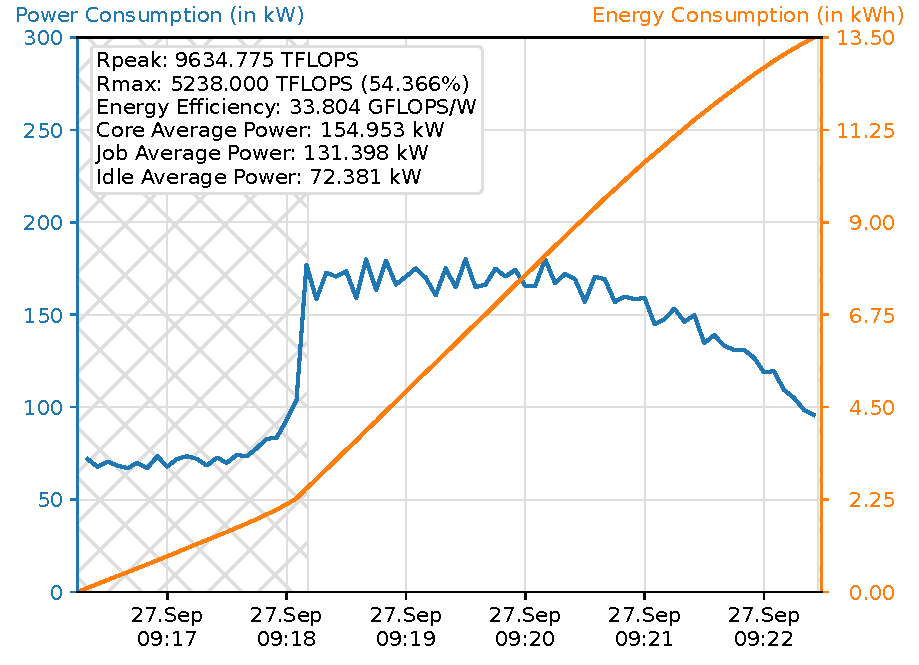
\includegraphics[width=0.75\textwidth]{data/example-rwth-claix-2023-gpu/summary.pdf}
    \caption{Summary of the CLAIX-2023 GPU Green500 submission. The hatched area indicates job execution outside the \acs{HPL} core phase.}
    \label{fig:example-rwth-claix-2023-gpu-summary}
\end{figure}
